\input{../../../../.preambles/02-lab_work}
\input{../../../../.preambles/20-math}
\newgeometry{top=1.5cm, bottom=1.5cm, left=1cm, right=1cm}
\begin{document}
    \makeheader{3}{Память \( 4\times1 \)}{Чечеткин И. А.}{Ф-369}{19.04.2013}
    
    \emph{Цель работы:} научиться работать со сложными элементами на примере
    RS-триггеров и составить схему памяти \( 4\times1 \) в программной среде
    \emph{Quartus}.

    \vspace*{2em}

    Схема памяти и ее временная диаграмма \(\bigl(\)адрес элементарной ячейки
    памяти \( A \) изменяется последовательно от 0 до~3, происходит смена
    уровня сигнала записи и чтения \emph{R/nW}, на вход \emph{data\_IN} данные
    для записи подаются случайным образом, вход \( C \)~-- синхросигнал, выходы
    \( Q_{00\ldots11} \)~-- состояния соответствующих элементарных ячеек, выход
    \emph{data\_OUT}~-- считанные данные\(\bigr)\) представлены на рисунке
    \ref{pic_memory}.
    
    \begin{figure}[h!]
        \center
        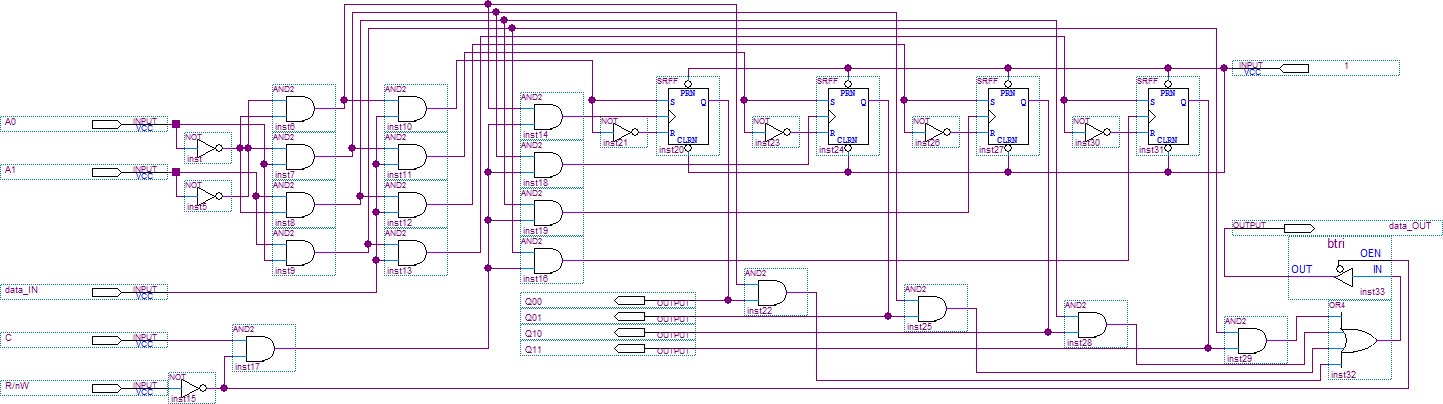
\includegraphics[width=1\textwidth]{sram} \vspace*{2em}\\
        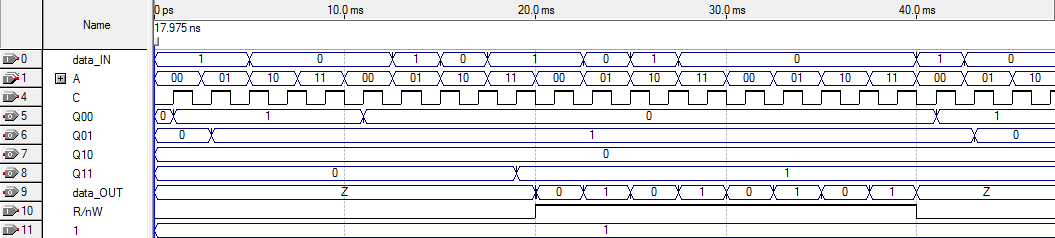
\includegraphics[width=.9\textwidth]{sram_time}
        \caption{Схема памяти и ее временная диаграмма}
        \label{pic_memory}
    \end{figure}    
\end{document}
